\documentclass{amia}
\usepackage[utf8x]{inputenc}
\usepackage{graphicx}
\usepackage{listings}
\usepackage[labelfont=bf]{caption}
\usepackage[superscript,nomove]{cite}
\usepackage{color}
\usepackage{caption}
\usepackage{todonotes}
\newcommand{\remPierre}[1]{\todo[color=green]{[PZ]{\scriptsize #1\par}}}
\newcommand{\remXavier}[1]{\todo[color=yellow]{[XT]{\scriptsize #1\par}}}
\newcommand{\remNico}[1]{\todo[color=orange]{[NP]{\scriptsize #1\par}}}


\newcommand\YAMLcolonstyle{\color{red}\mdseries}
\newcommand\YAMLkeystyle{\color{black}\bfseries}
\newcommand\YAMLvaluestyle{\color{blue}\mdseries}

\makeatletter

% here is a macro expanding to the name of the language
% (handy if you decide to change it further down the road)
\newcommand\language@yaml{yaml}

\expandafter\expandafter\expandafter\lstdefinelanguage
\expandafter{\language@yaml}
{
  keywords={true,false,null,y,n},
  keywordstyle=\color{darkgray}\bfseries,
  basicstyle=\YAMLkeystyle,                                 % assuming a key comes first
  sensitive=false,
  comment=[l]{\#},
  morecomment=[s]{/*}{*/},
  commentstyle=\color{blue}\ttfamily,
  stringstyle=\YAMLvaluestyle\ttfamily,
  moredelim=[l][\color{orange}]{\&},
  moredelim=[l][\color{magenta}]{*},
  moredelim=**[il][\YAMLcolonstyle{:}\YAMLvaluestyle]{:},   % switch to value style at :
  morestring=[b]',
  morestring=[b]",
  literate =    {---}{{\ProcessThreeDashes}}3
                {>}{{\textcolor{red}\textgreater}}1     
                {|}{{\textcolor{red}\textbar}}1 
                {\ -\ }{{\mdseries\ -\ }}3,
}

% switch to key style at EOL
\lst@AddToHook{EveryLine}{\ifx\lst@language\language@yaml\YAMLkeystyle\fi}
\makeatother

\newcommand\ProcessThreeDashes{\llap{\color{cyan}\mdseries-{-}-}}
\begin{document}


\title{i2b2 implemented over SMART-on-FHIR} 
\author{Nicolas Paris, MSc.$^{1}$,$^{2}$, Firstname B. Lastname, Degrees$^{2}$}

\institutes{
    $^1$WIND-DSI, AP-HP, Paris, France; $^2$LIMSI, CNRS, Université Paris-Saclay, Orsay, France; $^3$INSERM, UMR\_S 1142, LIMICS, Paris, France;\\
    }

\maketitle

\noindent{\bf Abstract}

\textit{Integrating Biology and the Bedside (i2b2) is the de-facto open-source medical tool for cohort discovery. Fast Healthcare Interoperability Resources (FHIR) is a new standard for exchanging health care information electronically. Substitutable Modular third-party Applications (SMART) defines the SMART-on-FHIR specification on how applications shall interface with  Electronic Health Records (EHR) thought FHIR. Related work made it possible to produce FHIR from an i2b2 instance or i2b2 to store FHIR datasets. In this paper, we extend i2b2 to search remotely into one or multiple SMART-on-FHIR Application Programming Interfaces (APIs). This enables the federation of queries, security, terminology mapping, and also bridges the gap between i2b2 and modern big-data technologies.}
%[h150  words]Programmatic themes: Translational
%Keywords: Cohort Discovery, Data integration and standardization, Informatics implementation

\section*{Introduction}
% A short background and objective(s) of the study

%\textit{FHIR} is becoming a standard for application to share EHR data and defines multiple resources representing multiple concepts (clinical, organisation\ldots). FHIR defines specification to. FHIR rapid success is partly du to the adoption of robust and widely used technologies such REST, json that made the success of internet major.
%
%\textit{SMART} success improve the user experience exaclty the same major internet provide access to many application with a single authentification.
%
%\textit{i2b2} is the de-facto open-source medical tool for cohort discovery and allows phisician to easily have translational view of their patients. Many initiatives have extended this primary goal with statistical analysis on place[ref], federating queries over multiple centers [shrine, insite, triknetX], and even genomics analytics.[transmart, i2b2-transmart]. It's recent migration on github makes possible multiple developpers to improve and extend the source code. I2b2 has been described to be used by more than 200 hospital over the world.
%The tool is flexible and can support its own stars schema and ontology model, or exploit OMOP common data model[]. Monthly ETL processes are generaly feeding the databases has time, resource, maintenance and disk space consuming processes. The database layer can be PostgreSQL, Oracle or Microsoft SQL Server. While those transfers in those relational databases are still feaseable these days, the emmergence of connected object and big-data generation let the methodology in the future incertain.
%
%This work is a general interface between i2b2 \& FHIR, exploiting the FHIR search[ref], Terminology Mapping[ref] and  SMART Oauth2 security[ref] specifications. The results does not only bridge the gap between two active communities, it opens to i2b2 new areas for data federation, data type hangling, security, interoperability and addresses the problem described above.
\remPierre{L'article actuellement fait trop ingénierie à mon avis. Il faudrait dans l'introduction commencer par établier les problèmes à résoudre (quelles sont les limitations des EHR actuels ?), puis indiquer des solutions envisagées ou testées dans les travaux antérieurs (...) et finir sur celle que tu proposes. L'évaluation devrait montrer dans quelle mesure ton travail résout les problèmes notés au départ.}
\remNico{j'ai fait les modifs suivantes dans le déroulé(je rajouterai une couche de vernis, si tant est que c'est mieux qu'avant): Objectif(learning health system);Solution actuelle(i2b2);problemes posés;solutions(FHIR);RelatedWork;Solution proposée.}
Learning Health Systems aim to maximize the potential of large-scale, harmonized data from variable, quickly-developing digital sources including Electronic Health Records (EHRs) emerging as powerful tools to facilitate discoveries that can improve health. Data heterogeneity is one of the critical problems in analyzing, reusing, sharing or linking datasets. With the development of platforms enabling the linking and federation of phenome, genome and exposome data across sites in US\cite{ref5,ref6} Europe\cite{ref7,ref8} or at international scale\cite{ref9} a key challenge is to define harmonized access to heterogeneous EHR-based data.

i2b2 is the de-facto open-source medical tool for cohort discovery and allows healthcare practitioners to easily subset patient data to address research questions. Many initiatives have extended this primary goal with statistical analysis on place, federating queries over multiple centers\cite{shrine,insite,trinetx} , and even genomics analytics.\cite{transmart,i2b2-transmart}. Its recent migration on github allows multiple developers to improve and extend the source code. I2b2 has been described to be used by more than 200 hospitals over the world. The tool is flexible and can support its own stars schema and ontology model, or exploit new information models e.g. PCORnet\cite{pcornet} or OMOP common data model\cite{ref14} - without requiring changes to the underlying data. 

i2b2 and derived solutions do have fields of improvement.  In terms of \textit{data variety}, each federation tools listed below proposes or not their own terminology mapping processes\cite{shrine}. When they exist\cite{ehr4crlesson}, they are time consuming and software specific\cite{i2b2map}.  In terms of \textit{freshness of the data}, Extract Transform Load processes (ETL) feeding the traditional relational databases supported by the tool (postgreSQL, Oracle, MSSQL) are time, resource, maintenance and disk space consuming. Though ETL are still feasible these days, the emergence of high throughput healthcare data and the Internet of Things requires the development of new approaches that allows querying data in place (directly in EHRs) or in optimized, dedicated places. This time delta due to data migrations and transformations poses problems of \textit{data veracity} because the source data is succeptible to be modified in the interval, and multiple transformation are error prone.  In terms of \textit{data volumetry}, data producer of interest for patient care such omics, exposomics, imaging or free text notes are challenging to store and also to analyse. They all need specialized and dedicated technology to be analysed properly and efficiently. While they have been several ingeniering attempts to make i2b2 based datawarhouses solution working with other technologies than traditional relational databases, the cost to create interfaces is high\cite{i2b2nosql}. The i2b2 star schema model, is highly optimized for fast retrieving lists of patients matching criteria. It is not intended for statistical analytics or data exploration\cite{i2b2export}. While they are some bridge with other common data-model [PCORNET, OMOP], the architecture is still based on RDBMS\cite{pcornet}The new technology emmergence is faster than i2b2 ability to exploit them.  In terms of \textit{software accessibility}, physician spend time switching from application, writing their login/password again \& again. Providing them the paradigm "one login/multiple applications" would paradoxaly improve the security, because this allow choosing a stronger password. Morover, this would optimize the time spent on computer and thus, improve patient care.

In the domain of patient care, several large-scale efforts have been underway for over a decade with the goal of specifying both the structure and the semantics of patient clinical information in a manner that enables computable semantic interoperability between diverse systems. Although there is no consensus in the medical informatics community regarding a standard patient information model, Health Level Seven (HL7) Fast Healthcare Interoperability Resources (FHIR) specifications are gaining interest and show promise to mitigate the classic site-specific data mapping problem. Built on lessons\cite{ref10} from previous standards including the Reference Information Model (RIM) that became an ISO standard in 2003 and Clinical Document Architecture, designed to express a single clinical document as a message using HL7 version 3 RIM classes. FHIR specifies a RESTful application programming interface (API) to access resources. Several initiatives facilitate the adoption of FHIR, including the Argonaut project\cite{ref11}, the Data Access Framework\cite{ref12} and the Clinical Information Modeling Initiative (CIMI)\cite{cimi}. 

SMART Health IT is an open, standards based technology platform that enables innovators to create apps that seamlessly and securely run across the healthcare system. Using an electronic health record (EHR) system or data warehouse that supports the SMART standard, patients, doctors, and healthcare practitioners can draw on this library of apps to improve clinical care, research, and public health (11. SMART success improve the user experience exaclty the same major internet provide access to many application with a single authentification.

Several work explored how to bridge i2b2 and FHIR. One approach\cite{apple} aims at allowing mobile phones to push FHIR resources into the i2b2 star schema. Other approaches\cite{wag,zappy} allow existing i2b2 instance to supply their star schema datasets as FHIR-API and allow to plug SMART-on-FHIR application on top of i2b2. The objectives of this work are to bring the latest accomplishments of the FHIR community to i2b2. In particular, bring the flexibility, the extensibility, the standardisation, and the interoperability efforts to i2b2.
This work describes a general interface between i2b2 and any type of clinical dataset derived by exploiting the FHIR search\cite{}, Terminology Mapping\cite{} and SMART Oauth2 security\cite{} specifications. The aim was not only to bridge the gap between patient care and research communities, but also to open to i2b2 new areas for better data types, security and interoperability management in the context of scalable solutions for cross border and cross domain networking of data. \remXavier{des exemples concrets de problèmes posés qui vont être résolus par ce travail ?}

\section*{Methods}
% Design, setting (if appropriate), patients or participants (if appropriate), interventions (if appropriate), and main outcome measurement

To meet the objectives, the existing i2b2 CRC cell code source is extended with code that meet the SMART-on-FHIR API specifications and the FHIR search API specifications. Figure \ref{fig1} \remXavier{attention aux labels des figures, la référence n'est pas bonne} shows the overall architecture and how the three-tier i2b2 application articulates with 3 remote institutions. The figure shows how i2b2 application gives access to users in a SMART-on-FHIR application context. In this context, users log one time in any SMART application or EHR, and get access to their specialized applications available. Moreover, the architecture allows to mix queries over multiples endpoints: zero to one i2b2 star schema and/or zero to many SMART-on-FHIR APIs.


Figure \ref{fig2} is a detailled UML. The scenario describes a user who query over an i2b2 instance with multiple remote FHIR-endpoints accesses. \remNico{mis des couleurs,  reste à préciser que tout ce qui concerne les instances SMART Authentication/FHIR API / EHR database}
The user first logs-in with its personnal secrets informations, that are verified by the i2b2 project management cell (i2b2pm). The i2b2pm then asks and stores a Oauth2 credential to all the SMART authentication services with it's own i2b2 connection details (one global secret for the i2b2 application) dedicated for the user\remXavier{Est-ce nécessaire de détailler l'authentification ?}. The i2b2pm returns then an i2b2 project list, to let the user choose and access according its habilitation details defined into i2b2. The user builds and run a multiple panel query accross different medical domains to get back a patient cohort set. The i2b2 query search module (i2b2crc) will then loop the following steps over each panel and each SMART-on-FHIR API. The i2b2crc transforms the query according to the FHIR-search specifications  and passes it with the credentials to the FHIR-API. The Oauth2 credential information are verified by the FHIR-API, and the query extended with the coding with synonyms defined in the terminology ConceptMap. The resulting query is then translated by the FHIR-API in the local database dialect to fetch the result. The result is transformed into a FHIR json bundle only containing the information needed (patient\_ids in this case). A parsing step extract the patient\_ids. They are mapped to an i2b2 unique identifier thanks to the existing i2b2 patient\_mapping features, to be then pushed into a CRC temporary table that integrates all the results. Once looping done, the i2b2crc applies the patients security steps to the CRC tmp table in order to only keep the patients that are available for the project selected by the user. The patient cohort set is finally returned to the user.\remXavier{Qu'est-ce qui est spécifique dans la "nouvelle" architecture ? le bleu de la figure ? pas clair}

\begin{figure}[h]
\centering
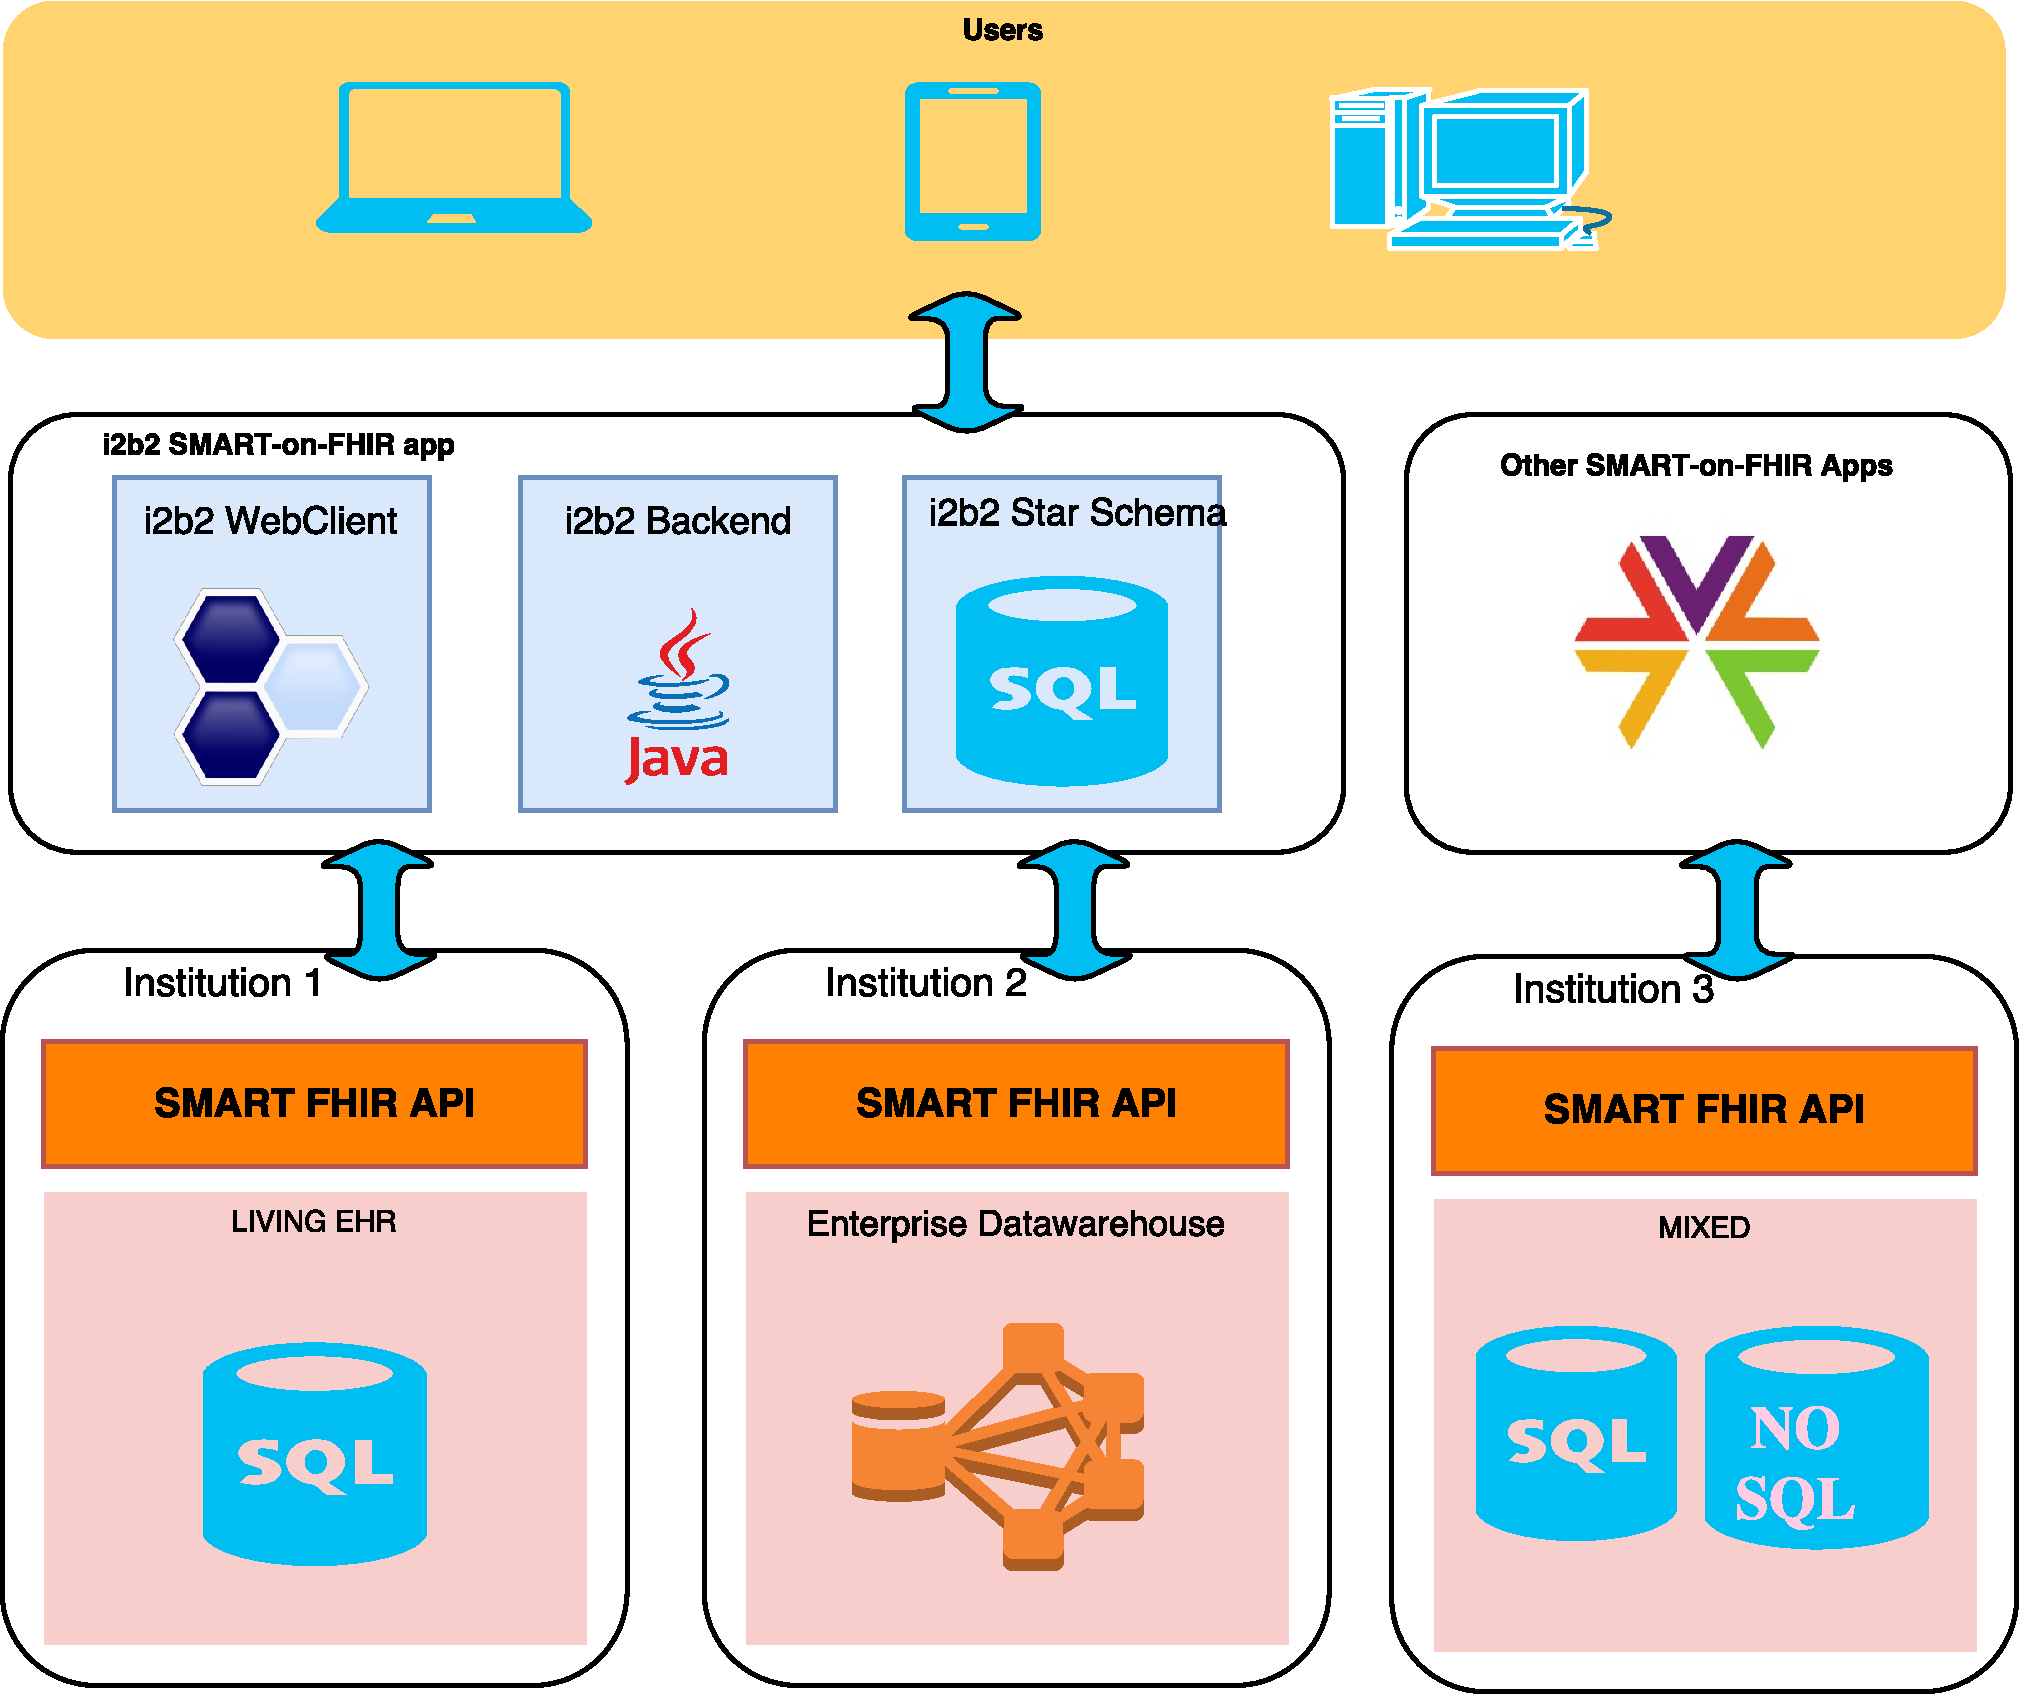
\includegraphics[scale=.4]{overall.pdf}
	\caption{Overall Diagram}
\label{fig1}
\end{figure}

\begin{figure}[h]
\centering
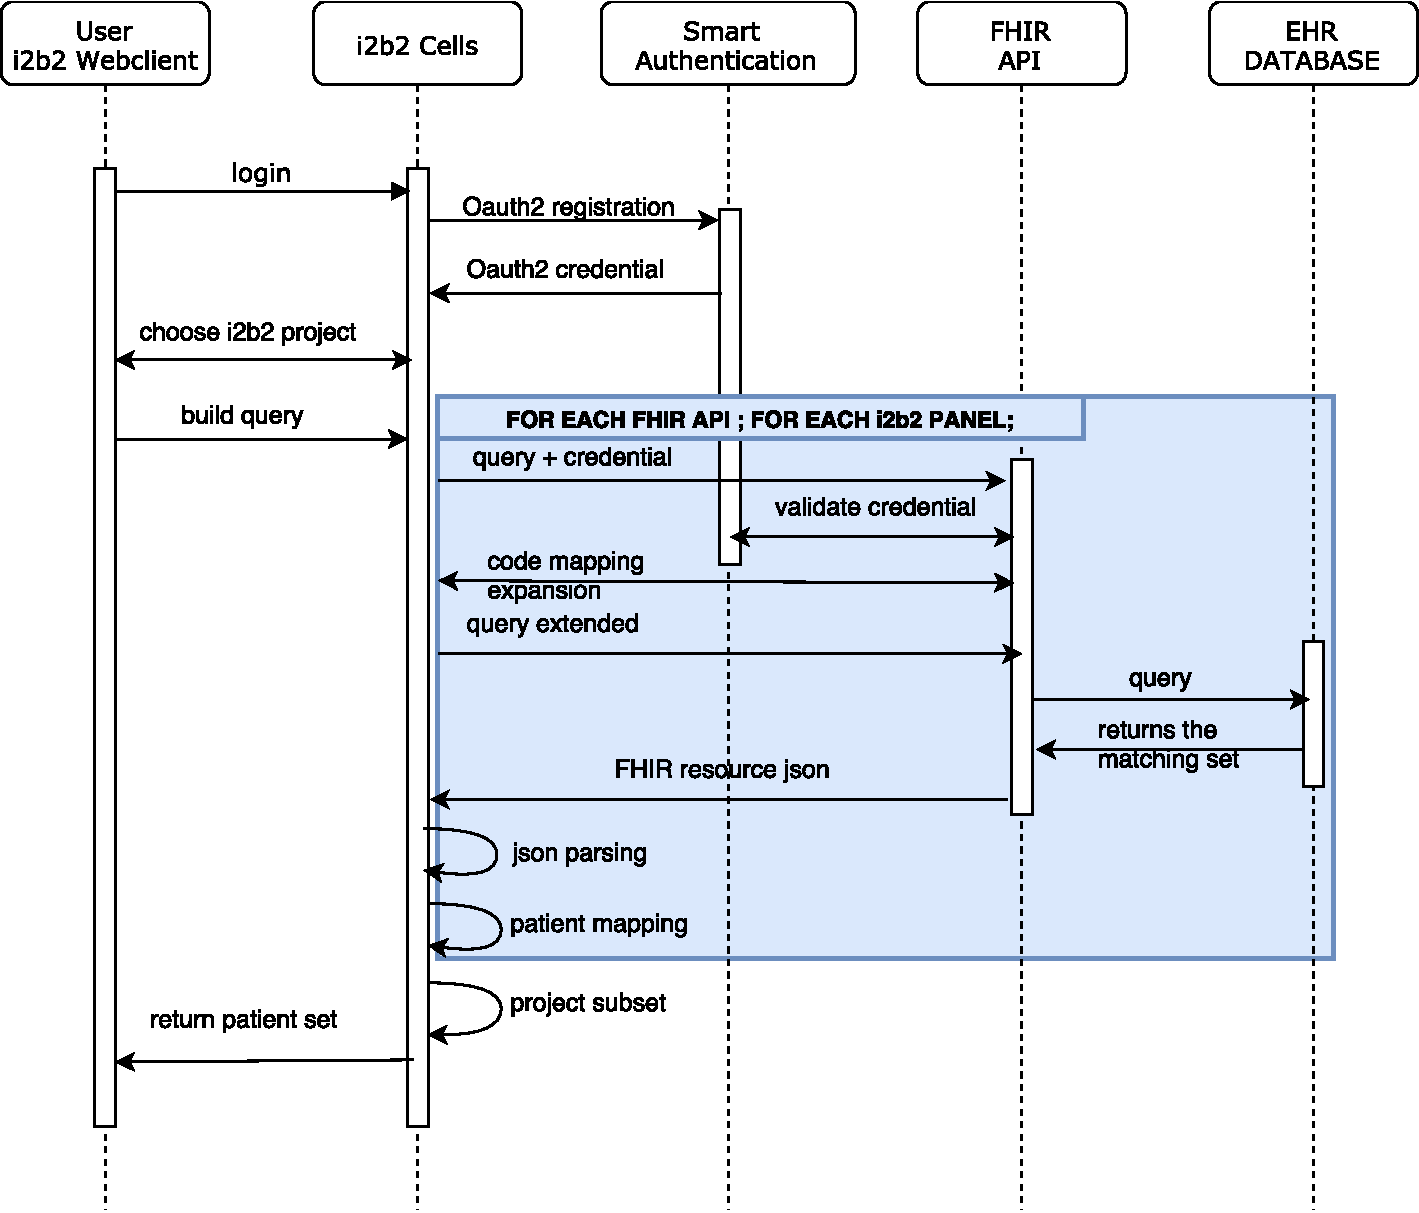
\includegraphics[scale=.5]{sequence_diagram.pdf}
\caption{UML Sequence Diagram}
\label{fig1}
\end{figure}

\begin{table}[h]
\centering
	\begin{tabular}{|p{6cm}|p{10cm}|}
  \hline
    \textbf{HTTP request}    & \textbf{Description}  \\ \hline
		GET $<$FHIR-API$>$/$<$Resource$>$\newline?\_elements=$<$elements$>$\&code=$<$codes$>$\newline\&date=gt$<$date\_inf$>$\&date=lt$<$date\_sup$>$\newline\&$<$custom\_filter$>$  & Retrieves choosen $<$elements$>$ from resources optionally matching a date range or/and a list of $<$codes$>$  or/and a $<$custom\_filter$>$     \\ \hline
	 GET $<$FHIR-API$>$/ConceptMap\newline?target-code=$<$codes$>$\newline\&target-system:in=$<$code-system$>$  & Retrieves all codes that are mapped to $<$codes$>$ \& $<$code-system$>$   \\ \hline
  \end{tabular}
\caption{Index of HTTP requests templates}
	\label{tab2}
\end{table}

\begin{table}[h]
\centering
	\begin{tabular}{|p{2cm}|p{6cm}|p{5cm}|}
  \hline
		\textbf{ontology table columns}    & \textbf{Description} & \textbf{Example} \\ \hline
		c\_basecode  &  FHIR code\_system / code pipe separated  & FHIR:http://loinc.com$|$1234-5  \\ \hline
		c\_facttable  &  Resource / Profile pipe separated  & Observation$|$ObservationAphp  \\ \hline
		c\_metadataxml  &  An xml describing datatype (numeric, free text or enumerated) and measure units  & cf: i2b2 documentation   \\ \hline
		c\_concept\_cd  &  an optionnal additional filter  & active=true\&status=final  \\ \hline
  \end{tabular}
\caption{i2b2 ontology adapted for FHIR}
	\label{tab1}
\end{table}

\begin{figure}
\begin{lstlisting}[language=yaml]
version: dstu3
Patient:
    patientUriPath: $.resource.id
    patientUriField: id
Observation:
  - patientUriPath: $.resource.subject.reference,
  - encounterUriPath: $.resource.context.reference
  - instanceUriPath: $.resource.id
  - datePath: $.resource.effectiveDateTime
  - patientUriField: subject
  - encounterUriField: context
  - instanceUriField: id
  - dateField: effective
[...]
\end{lstlisting}
  \caption{i2bé-FHIR resource YAML configuration file sample}
	\label{conf1}
\end{figure}
\textit{FHIR-search:} FHIR search specifications describe how to communicate with a FHIR-API to get back a set of resources matching an HTTP query criteria. The present work exploits only the possibility to fetch one type of resource per query. This is sufficient because i2b2 traditional query search module (i2b2crc) allows combining multiple filters predicates processing each separately and then uses a deliberation step using temporary tables. The idea of the query builder extension, is to be able to replace the i2b2crc SQL queries acting over the star schema to fetch record identifiers (ID) with HTTP calls to a FHIR-API and then any database system behind. The HTTP calls enabled in this design are presented in Table \ref{tab2}. The first row is the general template used, and has an analogy with SQL syntax:
\begin{itemize}
	\item[SELECT:] The $<$elements$>$ pattern lists the resource elements that are returned by the FHIR-API. Depending on the user choise, patient ID, encounter ID, instance ID or date are retrieved. The way to retrieve those information from a given resource is described into the i2b2 FHIR config YAML file Figure \ref{conf1}.
	\item[FROM:] The $<$Resource$>$ pattern is supposed to be replaced by any existing FHIR standard resource, or any profiled resource (modification of the standard to meet the local institutions constraints). In order to let the user point to the right RHIR resource, the i2b2 traditional ontology table has been reused and populated with the information. The Table \ref{tab1} describe how to store the information into the column "c\_facttable".
	\item [WHERE:] Both patterns $<$date\_inf$>$ and $<$date\_sup$>$ allows filtering the data based on date range. The $<$custom\_filter$>$ allows to combine a predefined pattern, such data status, or a user defined constraint by value query. The $<$codes$>$ pattern can optionally contain a list of coding (e.g: SNOMED, LOINC\ldots). Again, the i2b2 ontology table (Table \ref{tab1}) contains the codes informations in c\_basecode. While the date constraints are defined by the user at run time, they are not stored, the value constraint is enabled by filling the "c\_metadataxml" column, as described into the i2b2 documentation.\remXavier{un peu trop détaillé ?} \remNico{je vais clarifier voire simplifier}
\end{itemize}
\textit{FHIR-mapping:} The second row of the Table \ref{tab2} describes the HTTP query template to enable the terminology mapping. It is then possible to the i2b2crc to use this functionnality to fetch semantical synonyms that are described into the FHIR-Terminology server. As part of the ConceptMap\cite{ref15} resource, FHIR links a source code to a target with a set of semantic "equivalence" such "equivalent" or "narrower" that caracterize the way they relate together. The program fetches each mapping pairs and only keep the "wider", "subsumes", "equal", and "equivalent" semantic equivalence sources. The i2b2-FHIR code expansion exploits this mecanism to query over distinct codes systems.

%- sequence diagram (user, i2b2, i2b2 database, smart, EMR database)
%- Example of http queries produced by i2b2-fhir-search
%- Optimisation, ask only for elements needed by i2b2


\textit{Outcome measurement:} In order to test the FHIR DSTU3 resources compatibility coverage, the HAPI FHIR test server has been used as endpoint since it contains useful demo datasets for the 68 resources. The benchmark comparing traditional i2b2 and FHIR-i2b2 has been done with the same i2b2 observation\_fact table containing 140 million records in a postgresql 9.6 instance. The first is based on a 1.7 i2b2 instance. The FHIR-i2b2 has been setup by implementing HAPI-FHIR server on top of the observation\_fact table into an apache tomcat 9 webserver, and accessed via a the FHIR-i2b2 prototype. The FHIR-i2b2 big-data benchmark has been setup by implementing HAPI-FHIR server on top of a MIMIC3\cite{ref17} table multiplied by 15, and stored in a apache HIVE2 table distributed over a 5 computer cluster in ORC format.
All softwares used: i2b2, HAPI-FHIR, postgresql and apache Hive are open-source licensed.

\section*{Results}
% Key findings

\begin{figure}[h]
\centering
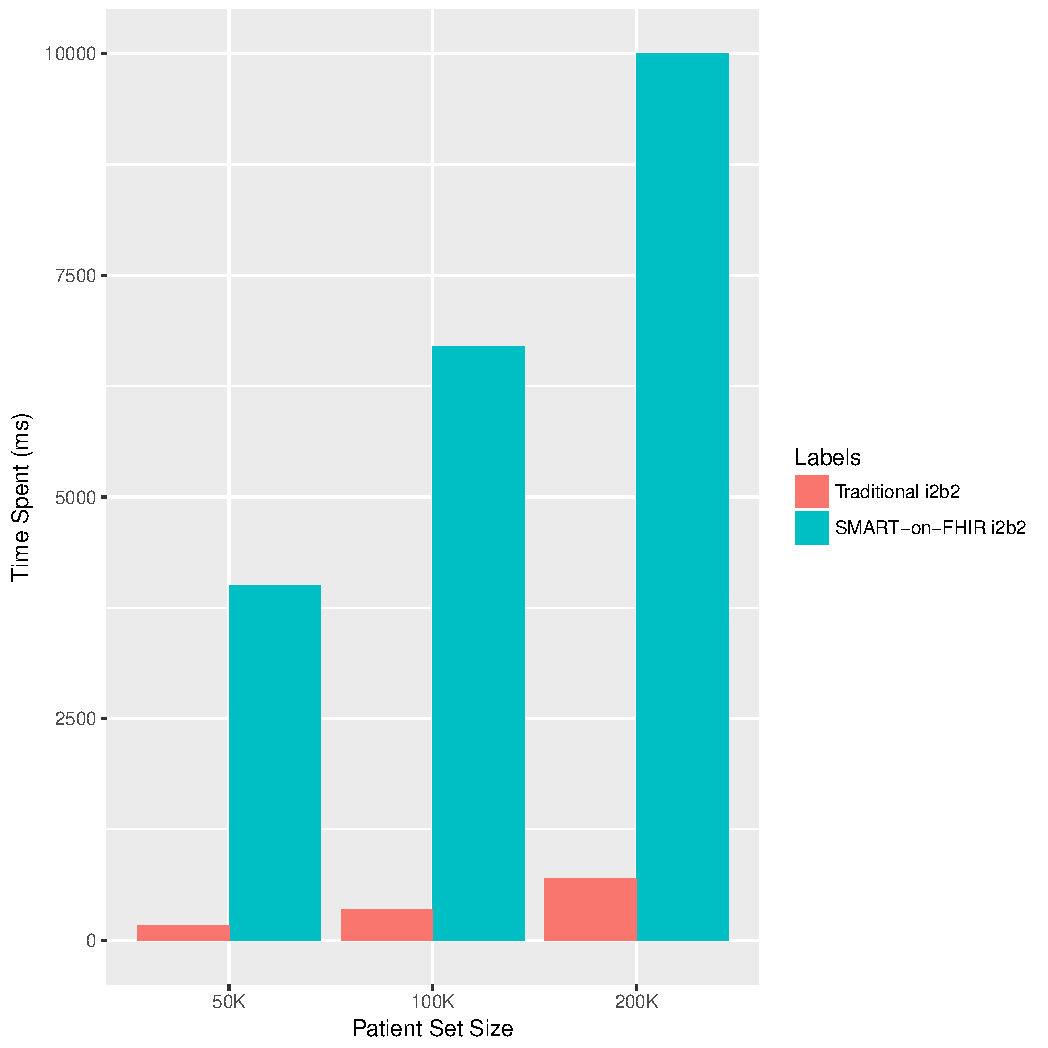
\includegraphics[scale=.7]{graph2.pdf}
	\caption{traditional versus SMART-on-FHIR performances comparison (on a 150M postgreSQL table)}
\label{fig1}
\end{figure}

\begin{figure}[h]
\centering
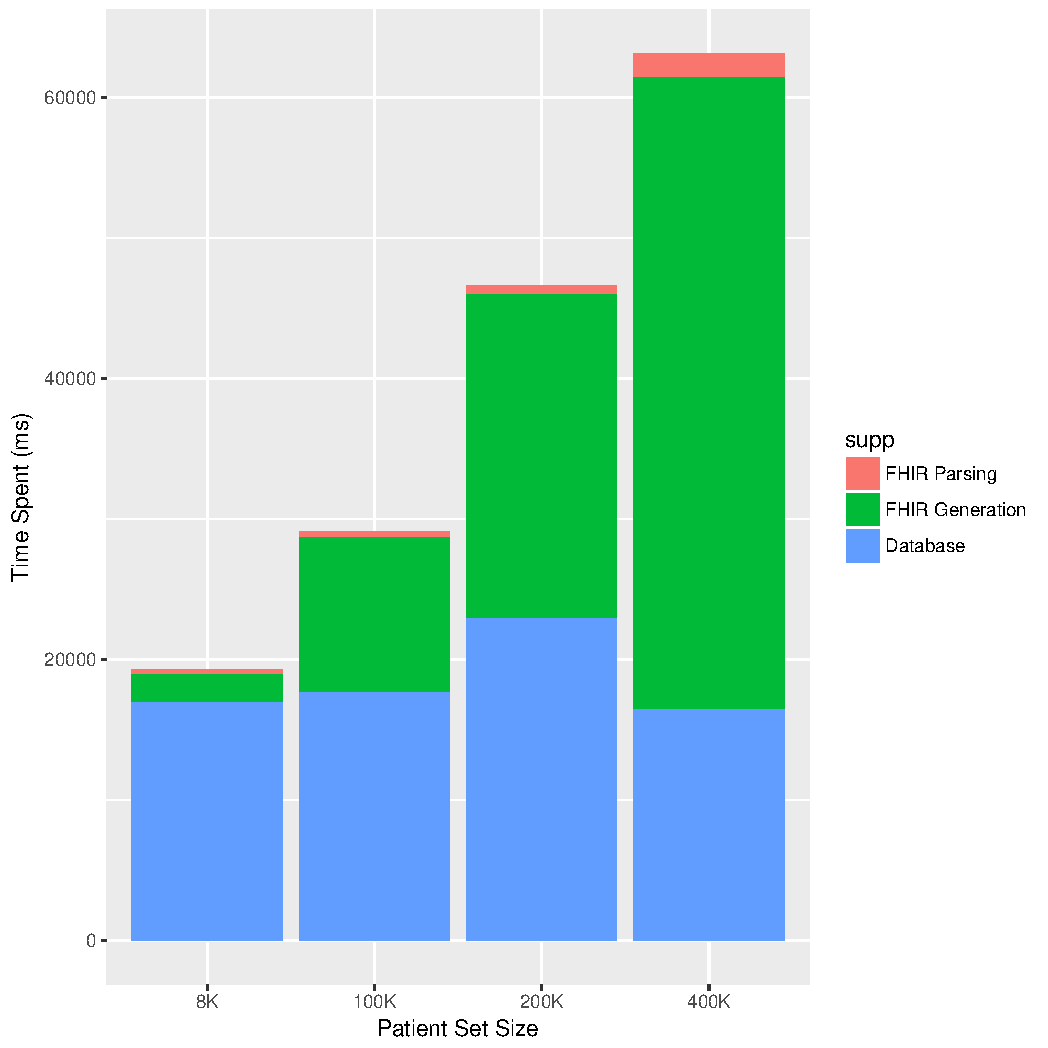
\includegraphics[scale=.7]{graph1.pdf}
	\caption{SMART-on-FHIR performances (on a 5B Hive table)}
\label{fig2}
\end{figure}
\begin{figure}[h]
\centering
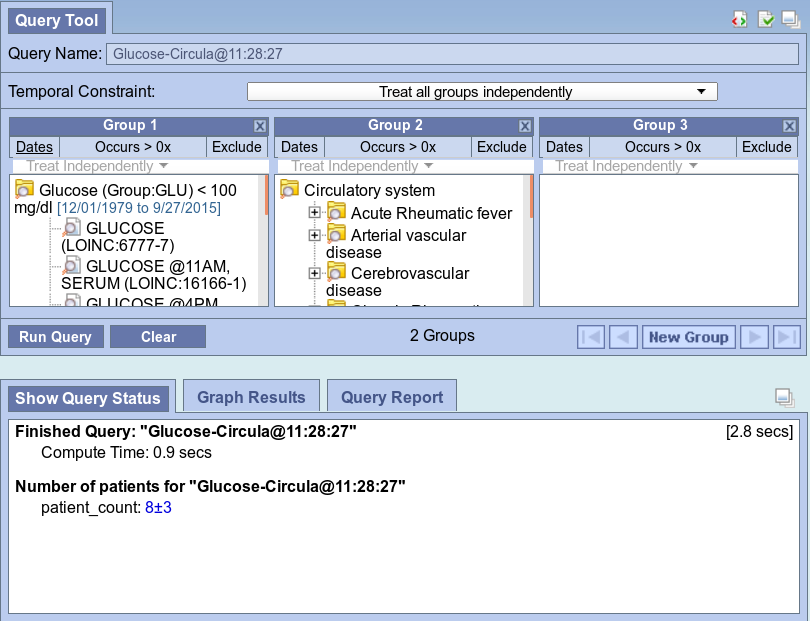
\includegraphics[scale=.5]{demo.png}
	\caption{SMART-on-FHIR online demo screenshot}
\label{fig3}
\end{figure}
\textit{Implementation Status: } The design presented below is not yet fully implemented\remPierre{Dire plutôt is implemented at XX\%}. To date, the query builder is able to query on both star schema and one remote FHIR endpoint simultaneously. Logical relation between selection criteria represented as multiple i2b2 webclient panels are also possible. The constitution of a patient\_set can be constraint by dates, by values and mesurement units and by one or multiple codes. The code expansion based on FHIR terminology mapping is also implemented. A living demo is deployed\cite{ref16}  and its screenshot presented in Figure \ref{fig3}. The panel 1 query searched into HAPI FHIR test server for patients with a set of loinc glucose codes having value lower than 100ml/dl in a year range from 1979 to 2015 and is mixed with the panel 2 searching for patients diagnosed related to circulatory system within the star schema. The resulting patient\_set is about 8 patients.

\textit{Performances: } The performances have been benchmarked (Figure \ref{fig1}) versus a traditional i2b2 instance based on star schema with the same amount of data, and configuration (140 Milion records). The histogram shows traditional i2b2 is 20 times faster than the i2b2-FHIR version. The difference can be explained by the additionnal steps involved: the fetched resultset is transformed into a json bundle, sent over the network and then parsed. The performance factor tends to decrease with number of patient matched. The second benchmark (Figure \ref{fig2}) experienced connecting to a apache HIVE table on a big-data platform. The results show that the time spent are under the minute and compatible with i2b2 promizes. Moreover, the barplots show that the major bottleneck is the FHIR json Generation step. Such amount of data have never been described to be handled by i2b2 before since we approach here traditional RDBMS limitations volumetry. While traditional i2b2 outperforms the FHIR based one on modest datasets, the latter opens new perspectives by allowing to connect to specialized and optimized database systems.


\textit{i2b2 feature coverage: }i2b2 querying feature covers filtering patients facts by code, values, dates, thought patient history, within an encounter temporal window or even a free sequence of events. By adding new temporal table mechanisms, the present work allows all those features. Ence, it does not limit the existing set of functionalities. The i2b2-FHIR configuration file Figure \ref{conf1} contains information about the FHIR-API instance, such its version, and how the resources are implemented. Depending on the kind of cohort set, the user want to extract, patient ID, encounter ID, instance ID or dates are retrived from the FHIR-API thanks to a jsonPATH description. This then allows to populate the CRC temporary tables. This is how i2b2 deliberation mecanisms can be populated, and the set build. The Table \ref{tab2} shows how those features are covered.

\textit{Security: }A security layer has been proposed and implemented into the existing CRC cell. A new i2b2 table allows to define witch patient are part of wich project. This security layer is important because it allows with one endpoint with all patients records, to create multiple projects with subset. In terms of performances, the table might be vertivally partitionned and splitted by project, in order to get stable performances while number of project will increase. This mecanism is both compatible with traditional i2b2 and i2b2-SMART-on-FHIR and has been deployed in production and handle more than distinct 200 projects.
The Oauth2 security layer has not yet been implemented. The implementation will inspire from project\cite{wag,apple} that recently succeed in.

\textit{Extensibility:} The FHIR access layer has been tested over the HAPI FHIR test server for all resources at least to refearing to a patient (68 resources), and does have a complete resource coverage. To date, the query builder is conpatible with last FHIR DSTU3 version. In the future, it will be compatible with each FHIR release, and maintain backward compatibilities. The FHIR version of each endpoint is setup in the configuration file (Figure \ref{conf1}). The query builder handles the FHIR extensibility, local profiled resources or even local new resources. Moreover, the design allows to filter based on FHIR extensions (https://www.hl7.org/fhir/extensibility.html\#extension). The results let conclude the design is flexible enougth to query multiple centers with different fHIR implementation at the same time.

\textit{Interoperability: }FHIR-ConceptMap expansion has been implemented. A set of test mapping have been produced and populated into HAPI-FHIR to make the proof of concept. The HTTP query described into Table \ref{tab2} allows to fetch the equivalent code. While their is some field of improvement, the results open area for massive and collaborative concept mapping, with a terminolgy server FHIR compatible. 
Interoperability is also derived from the FHIR standard resource difinition. However, the ability to derive from them and build Profiled Resources is catched by the i2b2-FHIR YAML configuration flexibility together with the i2b2 ontology table, as they are designed to be adapted.



\section*{Discussion}
\remNico{Compte tenue des problématiques évoqué en intro, je vais adapter discussion et conclusion}
% Key conclusions with direct reference to the foundational or methodological advancement or biomedical application
%- the performances open new area such Genomics\cite{ref4}, Imaging, Physiological Monitoring or even for i2b2 applications to discover new cohorts.
%- the security is renforced and allows multiple sub project to acces to subset of the whole patients. This addresses the patient research opposition and allows studies to only access to data they need. Moreover, it brings the last security technologies and allows federated architechture possible.
%- free text search: FHIR search specification covers filtering by dates, values or eaven basic operation on strings. However, it is not intended to allow text retrieval to mine the free-text notes. The abstraction provided by the FHIR layer allows to plug new text specific technologies based on apache lucene, such SOLR \& Elastic search. This will allow clinitian to mine text as simple as modern search engine does.
%- the interoperability gain from FHIR interface let envisage to query multiple center the same way on real-time data. This design allows two opposite paradigm. The first each clinitian is able to query i2b2 with it's own local terminologies he uses to code with. The second is to choose a Common Terminology Model as a pivotal, and map all the local coding to it. In both cases, the concept mapping remain to be done in many institution. Since all are based on different languages, different granularity and different concept and practices, this remains a challenge to be adressed.

FHIR abstraction allows designing mixed architecture based on living EHR and big-data storage to leverage massive and unstructured clinical data. One can choose the best technology depending on the expected usage and local specificity of the data. The flexible design allows implementers to define their own i2b2 ontologies. Finally, an i2b2 federation over FHIR is able to bridge multiple FHIR implementations at the same time. The querying benchmarks showed that performance was not an issue. Morover, by leveraging access to big-data technologies, this opens a new-area of specific solution to manage the diversity, variety and volumetry of healthcare data such Genomics, Imaging, Physiological Monitoring.

The abstraction provided by the FHIR layer allows plugging new text specific technologies based on apache lucene, such SOLR \& Elastic search. This will allow clinicians to mine text as simple as modern search engine does. - the interoperability gain from FHIR interface let envisage to query multiple center the same way on real-time data.
.The security was renforced and allows multiple sub projects to access to subsets of the whole patients database. This addresses the patient research opposition and allows studies to only access to data they need. Moreover, it brings the last security technologies and allows federated architechture possible. - free text search: FHIR search specification covers filtering by dates, values or eaven basic operation on strings. However, it is not intended to allow text retrieval to mine the free-text notes. 

Several modules have been implemented, some aspects of the design have only been tested as separate modules.
The roadmap provides for the development of multiple SMART-on-FHIR endpoints access, Oauth2 implementation and performances improvements. Once satisfied with the results, the system should be available in next releases of core i2b2. Specific exploration around specialized databases (temporal-series, text-mining, distributed, graph databases) will result to better handling variety of big-data, such genomic\cite{ref18}, textual notes, DICOM imaging, physiological waveforms or exposomic.

While all resource containing patient reference where tested, there is a need to propose a general mapping between traditional i2b2 objects (patient, visit, provider, observation) and FHIR specific resources (Organization, HealthcareService, Patient, EpisodeOfCare, Condition, Procedure, Medication, MedicationRequest, Observation, DiagnosticReport, ClinicalImpression\ldots)
A general algoritm to translate FHIR terminologies into i2b2 ontology will also be investigated, and result as a complementary sofware.

Last but not least concept mapping between many institutions and languages remains to be done. Since all are based on different languages, different granularity and different concept and practices, this remains a challenge to be adressed. While ontology matching has a long exp, this research area is still challenging.

\section*{Conclusion} 
\remXavier{on conclut avant de discuter ?}
\remNico{je m'étais fié au plan AMIA...}
The main contribution of the work is to pave the way for cohort-generation process by leveraging standard access, with interoperable terminology systems and state of the art security methods. The hospital centers international effort to converge to FHIR data exchange layer[ref] will ease the data-federation to query center without dedicated datawareouhsing staff. The main advantage over other approach to federate clinical repository such SHRINE, or Insite, is it benefits from FHIR ConceptMap and FHIR search that are already in place for other uses case in the institutions.
The secondary contribution of the work is to allow implementers to use their own technology, and allow i2b2 instance to benefits from the fast past and future improvements on big-data technologies.

Cross-border networking coordination and new technologies for data integration facilitates interoperability among research networks. Clinical research is on the threshold of a new era in which electronic health records (EHRs) are gaining an important novel supporting role. i2b2 has been extended to allow multicentric querying within research networks.  This paper proposed a new approach for linking i2b2 to EHRs.
%\section*{Conclusion}
%Your conclusion goes at the end, followed by References, which must follow the Vancouver Style (see: www.icmje.org/index.html).  References begin below with a header that is centered.  Only the first word of an article title is capitalized in the References. 
%\section*{Another Major Heading and References}
%This sentence has two reference citations\cite{ref1,ref2}.
%
%More text of an additional paragraph, with a figure reference (Figure ~\ref{fig1}) and a figure inside a Word text box below.  Figures need to be placed as close to the corresponding text as possible and not extend beyond one page.\\
%\begin{figure}[h]
%\centering
%\includegraphics[scale=1]{pics/figure1.png}
%\caption{Total allergy alerts, overridden alerts, or drug order cancelled.}
%\label{fig1}
%\end{figure}
%
%This is additional text added just to show the one-column formatting.  This is additional text added just to show the one-column formatting.  This is additional text added just to show the one-column formatting.  This is additional text added just to show the one-column formatting.  This is additional text added just to show the one-column formatting.  This is additional text added just to show the one-column formatting.  This is additional text added just to show the one-column formatting.
%
%This paragraph contains a reference to a table just below (Table 1).  All tables need to be placed as close to the corresponding text as possible, But each individual table should be on one page and not extend to multiple pages unless labeled as ``��Continued"��.
%
%\begin{table}[h]
%\centering
%\caption{Submission type, abstract length, and page length maximum for AMIA submissions.}
%  \begin{tabular}{|l|l|l|}
%  \hline
%    \textbf{Submission Type}    & \textbf{Abstract Length}  & \textbf{Page Length Maximum**} \\ \hline
%    Paper  & 125-150 words  & Ten   \\ \hline
%    Student Paper  & 125-150 words  & Ten \\ \hline
%    Poster  &50-75 words*   & One \\ \hline
%    Podium  Abstract & 50-75 words*  & Two \\ \hline
%    Panel   &150-200 words  & Three \\ \hline
%    System Demonstrations    &150-200 words  & One \\ \hline
%  \end{tabular}
%	\label{tab1}
%\end{table}
%*: All podium abstract and poster submissions must have a brief (50-75 words) abstract. The abstract does NOT have to be part of the document, but must be entered on the submission website in the Abstract box in Step 2.
%
%**: \textcolor{red}{If your submission is longer than what is specified below, it will be rejected without review.}
%
%This is another paragraph.


Voici des exemples de citations: MIMIC-III\cite{Johnson:SD2016} i2b2 \cite{Klann:JAMIA2016} et les références se mettent toutes seules dans la biblio ! Je pense que la référence vide numéro 1 vient d'un \verb+\cite{}+ avec argument vide.

\makeatletter
\renewcommand{\@biblabel}[1]{\hfill #1.}
\makeatother

\bibliographystyle{unsrt}
\bibliography{biblio}
\begin{thebibliography}{1}


\bibitem{transmart}
Scheufele E, Aronzon D, Coopersmith R, McDuffie MT, Kapoor M, Uhrich CA, et al. tranSMART: an open source knowledge management and high content data analytics platform. AMIA Summits on Translational Science Proceedings. 2014;2014:96. 

\bibitem{shrine}
Weber GM, Murphy SN, McMurry AJ, MacFadden D, Nigrin DJ, Churchill S, et al. The Shared Health Research Information Network (SHRINE): A Prototype Federated Query Tool for Clinical Data Repositories. Journal of the American Medical Informatics Association. 2009 Sep 1;16(5):624–30. 

\bibitem{ehr4crlesson}
Girardeau Y, Doods J, Zapletal E, Chatellier G, Daniel C, Burgun A, et al. Leveraging the EHR4CR platform to support patient inclusion in academic studies: challenges and lessons learned. BMC Medical Research Methodology [Internet]. 2017 Dec [cited 2017 Sep 28];17(1). Available from: http://bmcmedresmethodol.biomedcentral.com/articles/10.1186/s12874-017-0299-3

\bibitem{trinetx}
https://www.trinetx.com/

\bibitem{insite}
https://www.insiteplatform.com/

\bibitem{i2b2-transmart}
https://avillach-lab.hms.harvard.edu/

\bibitem{ref5}
Gottesman O, Kuivaniemi H, Tromp G, Faucett WA, Li R, Manolio TA, et al. The Electronic Medical Records and Genomics (eMERGE) Network: past, present, and future. Genet Med Off J Am Coll Med Genet. oct 2013;15(10):761--71.

\bibitem{ref6}
McMurry AJ, Murphy SN, MacFadden D, Weber G, Simons WW, Orechia J, et al. SHRINE: enabling nationally scalable multi-site disease studies. PloS One. 2013;8(3):e55811.

\bibitem{ref7}
De Moor G, Sundgren M, Kalra D, Schmidt A, Dugas M, Claerhout B, et al. Using electronic health records for clinical research: the case of the EHR4CR project. J Biomed Inform. Feb 2015;53:162--73. 

\bibitem{ref8}
Delaney BC, Curcin V, Andreasson A, Arvanitis TN, Bastiaens H, Corrigan D, et al. Translational Medicine and Patient Safety in Europe: TRANSFoRm--Architecture for the Learning Health System in Europe. BioMed Res Int. 2015;2015:961526. 

\bibitem{ref9}
Hripcsak G, Duke JD, Shah NH, Reich CG, Huser V, Schuemie MJ, et al. Observational Health Data Sciences and Informatics (OHDSI): Opportunities for Observational Researchers. Stud Health Technol Inform. 2015;216:574--8. 

\bibitem{ref10}
Rosenbloom ST, Carroll RJ, Warner JL, Matheny ME, Denny JC. Representing Knowledge Consistently Across Health Systems. Yearbook of Medical Informatics. 2017 Aug;26(01):139--47. 

\bibitem{pcornet}
Klann JG, Abend A, Raghavan VA, Mandl KD, Murphy SN. Data interchange using i2b2. Journal of the American Medical Informatics Association. 2016 Sep;23(5):909–15. 

\bibitem{ref17}
Johnson AEW, Pollard TJ, Shen L, Lehman LH, Feng M, Ghassemi M, et al. MIMIC-III, a freely accessible critical care database. Scientific Data. 2016 May 24;3:160035. 

\bibitem{ref14}
https://community.i2b2.org/wiki/display/OMOP/OMOP+Home

\bibitem{ref15}
https://www.hl7.org/fhir/conceptmap.html

\bibitem{ref16}
http://34.205.31.28/webclient/

\bibitem{apple}
Pfiffner PB, Pinyol I, Natter MD, Mandl KD. C3-PRO: Connecting ResearchKit to the Health System Using i2b2 and FHIR. Seo J-S, editor. PLOS ONE. 2016 Mar 31;11(3):e0152722. 

\bibitem{ref18}
Alterovitz G, Warner J, Zhang P, Chen Y, Ullman-Cullere M, Kreda D, et al. SMART on FHIR Genomics: Facilitating standardized clinico-genomic apps. Journal of the American Medical Informatics Association. 2015 Jul 21;ocv045. 

\bibitem{ref11}
HL7. HL7 Argonaut Project Wiki [Internet]. [cité 27 sept 2017]. Disponible sur: http://argonautwiki.hl7.org/index.php?title=Main\_Page

\bibitem{ref12}
\emph{To be provided (the Data Access Framework)}

\bibitem{ref1}
Pryor TA, Gardner RM, Clayton RD, Warner HR. The HELP system. J Med Sys. 1983;7:87-101.
\bibitem{ref2}
Gardner RM, Golubjatnikov OK, Laub RM, Jacobson JT, Evans RS. Computer-critiqued blood ordering using the HELP system. Comput Biomed Res 1990;23:514-28.

\bibitem{wag}
Wagholikar KB, Mandel JC, Klann JG, Wattanasin N, Mendis M, Chute CG, et al. SMART-on-FHIR implemented over i2b2. Journal of the American Medical Informatics Association. 2016 Jun 6;ocw079. 

\bibitem{zappy}
Boussadi A, Zapletal E. A Fast Healthcare Interoperability Resources (FHIR) layer implemented over i2b2. BMC Medical Informatics and Decision Making [Internet]. 2017 Dec [cited 2017 Sep 25];17(1). Available from: http://bmcmedinformdecismak.biomedcentral.com/articles/10.1186/s12911-017-0513-6

\bibitem{ref4}
Alterovitz G, Warner J, Zhang P, Chen Y, Ullman-Cullere M, Kreda D, et al. SMART on FHIR Genomics: Facilitating standardized clinico-genomic apps. Journal of the American Medical Informatics Association. 2015 Jul 21;ocv045. 

\bibitem{i2b2nosql}
Wang S, Pandis I, Wu C, et al. High dimensional biological data retrieval optimization with NoSQL technology. BMC Genomics. 2014;15(Suppl 8):S3. doi:10.1186/1471-2164-15-S8-S3.

\bibitem{cimi}
Mission and Goals | www.opencimi.org [Internet]. [cité 27 sept 2017]. Disponible sur: http://www.opencimi.org/

\bibitem{i2b2map}
Wynden R, Weiner MG, Sim I, Gabriel D, Casale M, Carini S, et al. Ontology mapping and data discovery for the translational investigator. Summit on Translational Bioinformatics. 2010;2010:66. 

\bibitem{i2b2export}
Firnkorn D, Merker S, Ganzinger M, Muley T, Knaup P. Unlocking Data for Statistical Analyses and Data Mining: Generic Case Extraction of Clinical Items from i2b2 and tranSMART. Stud Health Technol Inform. 2016;228:567-71.

\end{thebibliography}
\end{document}
